\documentclass[a4paper,12pt]{article}

\usepackage{mystyle}

\usepackage{gensymb}
\usepackage{scalerel}
\usepackage{stackengine}

% \usepackage{skull}  % skull
\usepackage{halloweenmath}  % \bigpumpkin, skull (https://tug.ctan.org/info/symbols/comprehensive/symbols-a4.pdf -- Table 76)

\usepackage{tikzsymbols}

% https://tex.stackexchange.com/questions/3266/how-do-i-use-a-circle-as-a-math-accent-larger-than-mathring
% https://tex.stackexchange.com/a/3270/135045
\usepackage{accents}

\renewcommand{\mathring}[1]{\accentset{\circ}{#1}}


\graphicspath{ {images/} }


% https://tex.stackexchange.com/questions/5461/is-it-possible-to-change-the-size-of-an-arrowhead-in-tikz-pgf
\usetikzlibrary{arrows.meta}


\DeclareMathOperator{\Image}{Im}

\definecolor{pink}{RGB}{218, 3, 174}
\definecolor{violet}{RGB}{148, 0, 211}
\definecolor{green}{RGB}{0, 153, 0}
\definecolor{orange}{RGB}{255, 153, 0}
\definecolor{blue}{RGB}{5, 73, 255}
\definecolor{cyan}{RGB}{31, 206, 203}
\definecolor{cyan2}{RGB}{0, 166, 147}
\definecolor{cyangreen}{RGB}{0, 155, 118}
\definecolor{cyangreen2}{RGB}{0, 109, 91}


% https://tex.stackexchange.com/a/101138/135045

\newcommand\widesim[1]{\ThisStyle{%
  \setbox0=\hbox{$\SavedStyle#1$}%
  \stackengine{-.1\LMpt}{$\SavedStyle#1$}{%
    \stretchto{\scaleto{\SavedStyle\mkern.2mu\sim}{.5150\wd0}}{.6\ht0}%
  }{O}{c}{F}{T}{S}%
}}


\newcommand{\BigMiddleTwo}{\;\left|\vphantom{\begin{pmatrix} 0\\0 \end{pmatrix}}\right.\;}
\newcommand{\BigMiddleThree}{\;\left|\vphantom{\begin{pmatrix} 0\\0\\0 \end{pmatrix}}\right.\;}
\newcommand{\BigMiddleFour}{\;\left|\vphantom{\begin{pmatrix} 0\\0\\0\\0 \end{pmatrix}}\right.\;}


% https://tex.stackexchange.com/questions/63531/how-to-write-quotation-marks-in-math-environment
\DeclareMathSymbol{\mlq}{\mathord}{operators}{``}
\DeclareMathSymbol{\mrq}{\mathord}{operators}{`'}

% TODO: didn't work...
% \renewcommand{\Re}{\mathop{\mathrm{Re}}\nolimits}
% \renewcommand{\Im}{\mathop{\mathrm{Im}}\nolimits}

\DeclareMathOperator{\Arg}{Arg}
\DeclareMathOperator{\Real}{Re}
\DeclareMathOperator{\Imag}{Im}


% https://tex.stackexchange.com/questions/544453/undefined-control-sequence-after-paragraph
\renewcommand{\paragraph}[1]{\noindent\textbf{#1}\quad}


% https://tex.stackexchange.com/questions/36851/skipping-line-after-proof-in-proof-environment#comment73553_36851
\newcommand{\proofindent}{\hspace*{\fill}\par\vspace{0.5em}\noindent}


% https://tex.stackexchange.com/questions/4813/extendible-equals-sign
\makeatletter
\newcommand*{\Relbarfill@}{\arrowfill@\Relbar\Relbar\Relbar}
\newcommand*{\xeq}[2][]{\ext@arrow 0055\Relbarfill@{#1}{#2}}
\makeatother


% https://tex.stackexchange.com/questions/279100/typeset-the-shrug-%C2%AF-%E3%83%84-%C2%AF-emoji
\newcommand{\shrug}[1][]{%
\begin{tikzpicture}[baseline,x=0.8\ht\strutbox,y=0.8\ht\strutbox,line width=0.125ex,#1]
  \def\arm{(-2.5,0.95) to (-2,0.95) (-1.9,1) to (-1.5,0) (-1.35,0) to (-0.8,0)};
  \draw \arm;
  \draw[xscale=-1] \arm;
  \def\headpart{(0.6,0) arc[start angle=-40, end angle=40,x radius=0.6,y radius=0.8]};
  \draw \headpart;
  \draw[xscale=-1] \headpart;
  \def\eye{(-0.075,0.15) .. controls (0.02,0) .. (0.075,-0.15)};
  \draw[shift={(-0.3,0.8)}] \eye;
  \draw[shift={(0,0.85)}] \eye;
  % draw mouth
  \draw (-0.1,0.2) to [out=15,in=-100] (0.4,0.95); 
\end{tikzpicture}}



% https://tex.stackexchange.com/a/314638/135045
% \newcommand{\diff}{\mathop{}\!d\!}
\newcommand{\diff}{\mathop{}\!d}


% https://tex.stackexchange.com/questions/387570/how-to-make-cdot-operator-same-width-as-division-slash-operator-and-vice-ve
\newcommand*{\slashdiv}{\makebox[\widthof{${}\cdot{}$}]{{}/{}}}


% https://tex.stackexchange.com/questions/9641/filled-diamondsuit-and-heartsuit
% https://tex.stackexchange.com/a/9643/135045
\DeclareSymbolFont{extraup}{U}{zavm}{m}{n}
\DeclareMathSymbol{\varheartsuit}{\mathalpha}{extraup}{86}
\DeclareMathSymbol{\vardiamond}{\mathalpha}{extraup}{87}
% https://tex.stackexchange.com/questions/234942/whats-the-best-way-to-make-a-heart-butt-in-latex
\newcommand{\heart}{\ensuremath\varheartsuit}


% https://tex.stackexchange.com/questions/247681/how-to-create-checkbox-todo-list
% https://tex.stackexchange.com/a/313337/135045
\usepackage{pifont}

\newlist{todolist}{itemize}{2}
\setlist[todolist]{label=$\square$}

\newcommand{\cmark}{\ding{51}}
\newcommand{\xmark}{\ding{55}}

\newcommand{\done}{\rlap{$\square$}{\raisebox{2pt}{\large\hspace{1pt}\cmark}}%
\hspace{-2.5pt}}
\newcommand{\failed}{\rlap{$\square$}{\large\hspace{1pt}\xmark}}




\author{Алексеев Василий}


\title{Семинар 3}
\date{21 февраля 2025}


\begin{document}
  \maketitle
  
  \tableofcontents

  \thispagestyle{empty}
  
  \newpage
  
  
  
  \vspace*{\fill}
  
  \noindent
  \emph{
    К формулировкам и доказательствам (если такие вообще приводятся) стоит относиться критически.
    Основное в этом конспекте~---~решение задач (но ``критичность'' и здесь лучше не отключать).
    За строгой, ясной и последовательной теорией лучше обращаться к ``нормальным'' источникам.
    (Например, к лекциям.)
  }
  
  \vspace*{\fill}
  
  \thispagestyle{empty}
  
  \newpage
  
  
  \pagenumbering{arabic}

  \section{Эрэн}

  % [X] Векторы
  % [X] Операции (сложение + умножение на число) -> линейное пространство
  % [X] Расстояние -> метрическое пространство
  % [X] Окрестность
  % [X] Классификация точек по окрестности 1 (внутренние, изолированные, граничные)
  % [X] Сходимость (предел) (+ теоремы?)
  % [X] Классификация точек по окрестности 2 (предельные, прикосновения)

  \subsection{Множества}

  Элементы $\RR^n$~---~это $n$-мерные числовые \emph{векторы}:
  \[
    \bds x \in \RR^n \Rightarrow \bds x = (x_1, \ldots, x_n),\ x_i \in \RR
  \]
  при этом составляющие вектора называются его компонентами, или координатами.\footnote{
    В базисе $\bds e_1 \hm= (1, 0, \ldots, 0)$, ..., $\bds e_n \hm= (0, 0, \ldots, 1)$.
  }
  Сам вектор также будем называть \emph{точкой}.

  На множестве векторов~$\RR^n$ можно ``естественным''~---~покомпонентным~---~образом ввести операции сложения и умножения вектора на число (начиная отсюда и далее будем для простоты и большей наглядности использовать размерность $n \hm= 2$, хотя всё остаётся верным и для произвольного $n \in \NN$):
  \[
    \begin{aligned}
      &(x_1, y_1) + (x_2, y_2) = (x_1 + x_2, y_1 + y_2)\\
      &\alpha \cdot (x, y) = (\alpha \cdot x, \alpha \cdot y),\quad \alpha \in \RR
    \end{aligned}
  \]

  Можно проверить, что таким образом введённые операции удовлетворяют ряду ``привычных'' аксиом,\footnote{
    Эти аксиомы (четыре чисто про сложение + четыре про сложение и умножение):
    \begin{enumerate}
      \item $\bds x + (\bds y + \bds z) = (\bds x + \bds y) + \bds z$ (ассоциативность)
      \item $\bds x + \bds y = \bds y + \bds x$ (коммутативность)
      \item $\exists \bds 0\colon \bds x + \bds 0 = \bds x,\ \forall \bds x$
      \item $\forall \bds x\ \exists (-\bds x)\colon \bds x + (-\bds x) = \bds 0$
      \item $\alpha (\beta \bds x) = (\alpha \beta) \bds x$
      \item $1 \cdot \bds x = \bds x$ ($1$~---~просто единица, число из $\RR$)
      \item $\alpha (\bds x + \bds y) = \alpha \bds x + \alpha \bds y$ (дистрибутивность умножения вектора на число относительно сложения векторов)
      \item $(\alpha + \beta) \bds x = \alpha \bds x + \beta \bds x$ (дистрибутивность умножения вектора на число относительно сложения чисел)
    \end{enumerate}
  } поэтому множество векторов вместе с этими операциями $\langle\RR^n, +, \cdot\rangle$ образуют \emph{линейное пространство}.

  Кроме того, чтоб выполнять операции с векторами, можно бы было их каким-то образом \emph{сравнивать} между собой по \emph{близости}~---~оценивая \emph{расстояние}~$\rho$ между ними.
  В качестве расстояние можно взять, например, евклидово:
  \[
    \rho\bigl((x_1, y_1), (x_2, y_2)\bigr) = \sqrt{(x_1 - x_2)^2 + (y_1 - y_2)^2}
  \]

  Можно проверить, что таким образом введённое расстояние удовлетворяет ряду ``привычных'' аксиом,\footnote{
    Эти аксиомы:
    \begin{enumerate}
      \item $\rho(\bds x, \bds y) \geq 0$, $\rho(\bds x, \bds x) = 0 \Leftrightarrow \bds x = \bds 0$
      \item $\rho(\bds x, \bds y) = \rho(\bds y, \bds x)$ (симметричность)
      \item $\rho(\bds x, \bds z) \leq \rho(\bds x, \bds y) + \rho(\bds y, \bds z)$ (неравенство треугольника)
    \end{enumerate}
  } поэтому множество векторов вместе с такой функцией расстояния $\langle\RR^n, \rho\rangle$ образуют \emph{метрическое пространство}.\footnote{
    Это не единственный возможный способ ввести расстояние в~$\RR^n$.
    Например, можно бы было использовать манхэттенское расстояние:
    \[
      \rho_m\bigl((x_1, y_1), (x_2, y_2)\bigr) = |x_1 - x_2| + |y_1 - y_2|
    \]

    (Более того, манхэттенское расстояние в некотором смысле \emph{эквивалентно} евклидовому.
    Подробнее можно см. \href{https://mipt.ru/institute-departments/kafedra-vysshey-matematiki/study_docs/books_lections}{``Добавление к лекциям по математическому анализу'' за 1 семестр Балашова\,М.\,В.}, раздел <<Эквивалентность норм в $\RR^n$>> (норма~---~это как длина вектора), а также небольшое \href{https://math.stackexchange.com/questions/172028/difference-between-norm-and-distance}{обсуждение на Math Stack Exchange} про то, что норма и расстояние, хоть и связаны, но не всегда.
    (Поэтому из эквивалентности норм в $\RR^n$ не следует вообще эквивалентность всех расстояний.))

    Или дискретное:
    \[
      \rho_d(\bds x, \bds y) = \left\{
        \begin{aligned}
          1,\quad \bds x \not= \bds y\\
          0,\quad \bds x = \bds y
        \end{aligned}
      \right.
    \]

    Или ещё какое-нибудь.
  }

  Далее будем работать в метрическом пространстве $\langle\RR^n, \rho\rangle$.

  Имея возможность оценивать расстояние между векторами, можно ввести понятие \emph{окрестности} вектора:
  \[
    U_{r}(\bds a) = \{\bds x \in \RR^n \mid \rho(\bds x, \bds a) < r\}
  \]
  так можно обозначить окрестность вектора $\bds a$ радиуса $r \hm> 0$~(\ref{fig:vector-neighbourhood}).
  Таким образом, это множество векторов, удалённых от данного на расстояние меньше~$r$~---~то есть по сути \emph{шар} (без границы).
  ``Соседство'' вектора.

  \begin{figure}[ht]
    \centering
  
    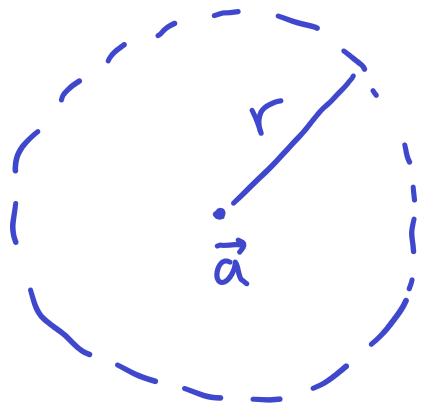
\includegraphics[width=0.25\columnwidth]{vector-neighbourhood}
  
    \caption{
      Окрестность $U_{r}(\bds a)$~---~множество точек, удалённых от~$\bds a$ на расстояние ближе~$r$.
    }
    \label{fig:vector-neighbourhood}
  \end{figure}

  Анализируя окрестности точек некоторого множества $X \hm\subseteq \RR^n$, можно выделить следующие ``категории'' точек~(\ref{fig:vector-types-by-neighbourhood}).

  \begin{definition}
    \emph{Внутренней точкой} множества $X \subseteq \RR^n$ называется такая точка $\bds x$, принадлежащая~$X$, что вокруг неё можно найти окрестность, целиком лежащую в~$X$:
    \[
      \exists \eps > 0\colon U_{\eps}(\bds x) \subseteq X \quad\Leftrightarrow\quad U_{\eps}(\bds x) \cap X = U_{\eps}(\bds x)
    \]
  \end{definition}

  \begin{definition}
    \emph{Изолированной точкой} множества $X \subseteq \RR^n$ называется такая точка $\bds x$, принадлежащая~$X$, что вокруг неё можно найти окрестность, не содержащую ни одной точки~$X$ (кроме самой~$\bds x$):
    \[
      \exists \eps > 0\colon U_{\eps}(\bds x) \cap X = \bds x
    \]
  \end{definition}

  \begin{definition}
    \emph{Граничной точкой} множества $X \subseteq \RR^n$ называется такая точка $\bds x$, возможно, принадлежащая~$X$, возможно, нет, что любая её окрестность содержит как точки~$X$, так и точки, не принадлежащие~$X$:\footnote{
      Иными словами, содержит как точки~$X$, так и точки его \emph{дополнения}: $\overline{X} \hm\equiv \RR^n \hm\setminus X$.
    }
    \[
      \forall \eps > 0 \to \left\{
        \begin{aligned}
          &U_{\eps}(\bds x) \cap X \not= \noth\\
          &U_{\eps}(\bds x) \not\subseteq X
        \end{aligned}
      \right.
    \]
  \end{definition}

  Очевидно, изолированные точки множества~$X$ будут также и граничными для него.\footnote{
    На самом деле не всегда: такая логика работает только в том случае, когда в качестве ``всего пространства'' рассматривается $\RR^n$.
    Но метрическое пространство~---~это не обязательно всё $\RR^n$.
    (Метрическое пространство~---~это просто какое-то множество векторов + функция расстояния между ними.)
    И если смотреть на множество точек~$X$~---~как на множество в каком-то метрическом пространстве, отличном от $\RR^n$, то тогда могут возникать некоторые дополнительные ``интересности''.

    В том числе, изолированная точка множества~---~не обязательно будет граничной.
    
    Пример: прямая $R$, на ней можно в качестве метрического пространства взять $M \hm= [0, 1] \hm\cup \{2\}$ (с обычным расстоянием).
    Если в таком пространстве теперь рассмотреть множество из одной точки $X = \{2\}$, то эта точка будет изолированной для $X$ в $M$, но не граничной (достаточно близко вокруг $2$ в пространстве $M$ просто ``пусто''~---~нет точек, не принадлежащих $X$).
    
    (Получается, у такого $X$ в $M$ не будет ни внутренних, ни граничных точек?)
    
    Ещё сколько-то примеров и в таком духе наблюдений можно найти в \href{http://math.phys.msu.ru/data/129/lec04a.pdf}{конспекте лекций по метрическим пространствам}.
  }\textsuperscript{,}\footnote{
    Если проводить аналогию с машинным обучением, то изолированная точка множества~---~это как выброс, какое-то ``экстремальное значение'', нетипичный представитель.
    Внутренняя точка~---~это, наоборот, что-то типовое, обычное.
    Граничная~---~...что-то ``непонятное'', ``ненадёжное'', может, тут, а может, тут.

    Например, в семье тупоконечников, тупоконечник~---~это типичный представитель (внутренняя точка).
    Остроконечник~---~``изгой'', не такой, как все (изолированная).
    А если человеку без разницы, с какого конца быть (бить), сегодня так, завтра, может, по-другому~---~то он ``никакой'' (граничная).
  }

  \begin{definition}\label{def:touch-point}
    \emph{Точкой прикосновения} множества $X \subseteq \RR^n$ называется такая точка $\bds x$, возможно, принадлежащая~$X$, возможно, нет, что любая её окрестность содержит точки~$X$:
    \[
      \forall \eps > 0 \to U_{\eps}(\bds x) \cap X \not= \noth
    \]
  \end{definition}

  Очевидно, внутренние точки, изолированные, граничные~---~являются точками прикосновения.
  (Есть ли ещё варианты ``прикосновения'', кроме этих?)

  Помимо выделения таких интересных классов точек, возможность оценивать расстояние даёт возможность ввести в~$\RR^n$ понятие \emph{предела последовательности}.

  Пределом последовательности $n$-мерных векторов $\{\bds x^{(m)}\}_{m = 1}^\infty$ называется вектор $\bds a$, такой что:\footnote{
    Индекс элемента последовательности указан сверху, да ещё и в ``каких-то непонятных'' скобках только по ``техническим причинам'': для того, чтобы избежать путаницы с индексами координат вектора.
  }
  \begin{equation}\label{eq:seq-limit}
  \begin{split}
    \forall \eps > 0\ \exists M > 0\colon \forall m \geq M &\to \rho(\bds x^{(m)}, \bds a) < \eps\\
      &\Leftrightarrow \bds x^{(m)} \in U_{\eps}(\bds a)
  \end{split}
  \end{equation}

  Можно заметить, что такое определение предела работает также и для рассмотренного ранее в курсе ``более простого'' случая точек на прямой~$\RR$~---~просто тогда расстояние будет считаться как модуль разности между числами: $\rho(x, a) \hm= |x - a|$.\footnote{
    Таким образом, точки на~$\RR$ и в~$\RR^n$ в некотором смысле поддерживают общий ``предельный интерфейс'': общее определение предела работает всегда, просто конкретная ``реализация'' участвующего в нём расстояния может быть разной.
  }

  Относительно сходимости последовательностей векторов в~$\RR^n$ также остаются верными некоторые утверждения, работающие для точек на~$\RR$.
  Но так как для решения задач они не понадобятся, то мы их упоминать не будем.\footnote{
    Подробнее можно см. хотя бы теорсправку в С3, \S 1.
  }

  Вооружившись понятиями сходимости и предела, можем продолжить ``классификацию'' точек множества $X \hm\subseteq \RR^n$.

  \begin{definition}
    \emph{Предельной точкой} множества $X \subseteq \RR^n$ называется такая точка $\bds x$, возможно, принадлежащая~$X$, возможно, нет, что любая её \emph{проколотая} окрестность содержит точки~$X$:\footnote{
      ``Предельность'' точки связана с ``проколотостью'' окрестности так: раз в любой проколотой окрестности можно найти точку $X$, отличную от самой $\bds x$, то можно построить сходящуюся к $\bds x$ последовательность точек~$X$ (уменьшая радиус окрестности и каждый раз выбирая из неё новую точку~---~расположенную всё ближе к~$\bds x$).
    }
    \[
      \forall \eps > 0 \to \mathring U_{\eps}(\bds x) \cap X \not= \noth
    \]
  \end{definition}

  Очевидно, предельные точки~---~это почти как точки прикосновения~(\ref{def:touch-point}), но с дополнительным ограничением~---~которое, очевидно, приводит к тому, что изолированные точки предельными не будут.

  \begin{figure}[ht]
    \centering
  
    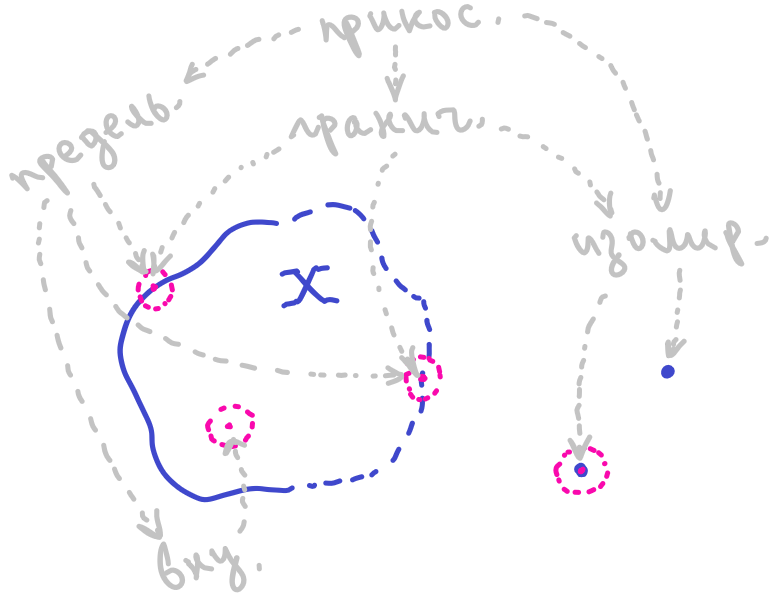
\includegraphics[width=0.8\columnwidth]{vector-types-by-neighbourhood}
  
    \caption{
      ``Классификация'' точек множества $X \hm\subseteq \RR^n$ в зависимости от расположения относительно~$X$.
    }
    \label{fig:vector-types-by-neighbourhood}
  \end{figure}

  \medskip

  Мы рассмотрели несколько типов точек в~$\RR^n$ (``микроопределения'').
  Введём ещё несколько типов множеств в~$\RR^n$ (``макроопределения'').
  (Типов~---~в зависимости от составляющих множества точек.)

  % \operatorname{int}

  \begin{definition}
      \emph{Открытым} множеством $X \subseteq \RR^n$ называется множество, все точки которого внутренние.

      Множество внутренних точек множества $X$ называется \emph{внутренностью} множества и обозначается как $\operatorname{int} X$.

      Таким образом, открытое~---~это такое~$X$, что:\footnote{
        Точнее, единственное, что надо требовать, это: $X \subseteq \operatorname{int} X$
      }
      \[
        X = \operatorname{int} X
      \]
  \end{definition}

  \begin{definition}
      \emph{Замкнутым} множеством $X \subseteq \RR^n$ называется множество, которое содержит все свои точки прикосновения.

      Множество точек прикосновения множества $X$ называется \emph{замыканием} множества и обозначается как $\overline X$.

      Таким образом, замкнутое~---~это такое~$X$, что:\footnote{
        Точнее, единственное, что надо требовать, это: $\overline X \subseteq X$
      }
      \[
        \overline X = X
      \]
  \end{definition}

  \begin{example}
    На прямой~$\RR$ открытыми множествами будут, например, интервалы, замкнутыми~---~отрезки.

    Окрестность точки в $\RR^n$~---~также пример открытого множества.

    Всё пространство~$\RR^n$ и пустое множество~$\noth$~---~примеры (единственные?) одновременно открытых и замкнутых множеств.
  \end{example}

  Открытые и замкнутые множества могут быть ``цельными''.
  Например, открытое $(0, 1) \hm\subset \RR$, замкнутое $[0, 1] \hm\subset \RR$.
  А могут быть ``разбиты'' на несколько обособленных, не связанных друг с другом частей.
  Например, открытое $(0, 1) \hm\cup (2, 3) \subset \RR$ или замкнутое $[0, 1] \hm\cup [2, 3] \subset \RR$.
  Свойство ``цельности'' можно сформулировать так.

  \begin{definition}
      Множество $X \hm\subseteq \RR^n$ называется \emph{линейно связным}, если любую пару точек множества~$X$ можно соединить непрерывной кривой (содержащейся во множестве).\footnote{
        Возможно (но не точно), что ``линейно связное'' надо понимать в том смысле, что между любой парой точек можно провести ``линию''.
        Непрерывная кривая, линия...
        ``Принимаемо''.
        
        В английском же это называется \href{https://en.wikipedia.org/wiki/Connected_space\#Path_connectedness}{path-connected}~---~``путесвязное множество''.
        Это более сильное свойство, чем ``просто'' связность, которая про то, представимо или нет данное множество как объединение двух или более непересекающихся открытых множеств (непустых).  % также см. https://bigenc.ru/c/sviaznoe-mnozhestvo-0365f0
        На первый взгляд может показаться, что разницы между такими ``связностями'' особо как будто и нет.
        Оказывается, что в некотором приближении так и есть: на числовой прямой $R$ связность просто эквивалентна ``путесвязности''; в $R^n$ же \emph{открытое} множество \href{https://en.wikipedia.org/wiki/Connected_space\#Path_connectedness}{связно тогда и только тогда, когда оно ``путесвязно''}.
        Но примеры, иллюстрирующие разницу между понятиями связности, тоже \href{https://w.wiki/DGXV}{при желании можно придумать}.
      }
  \end{definition}

  И отдельно выделяется класс ``цельных'' открытых множеств.

  \begin{definition}
    Множество $X \hm\subseteq \RR^n$ называется \emph{областью}, если оно открыто и линейно связно.
  \end{definition}

  В классификации множеств можно пойти ещё дальше: среди ``цельных'' можно выделить ``размазанные'' (``амёбеобразные'') и ``плотно упакованные''~(\ref{fig:ameba-and-convex}).

  \begin{figure}[ht]
    \centering
    
    \begin{subfigure}[b]{0.3\textwidth}
      \centering
    
      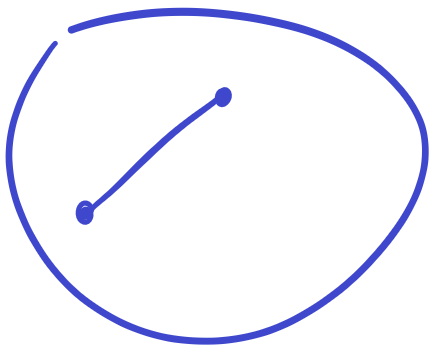
\includegraphics[width=\columnwidth]{convex-example}
    
      \caption{Выпуклое.}
    \end{subfigure}
    %
    \hspace{2em}
    %
    \begin{subfigure}[b]{0.3\textwidth}
      
      \centering
      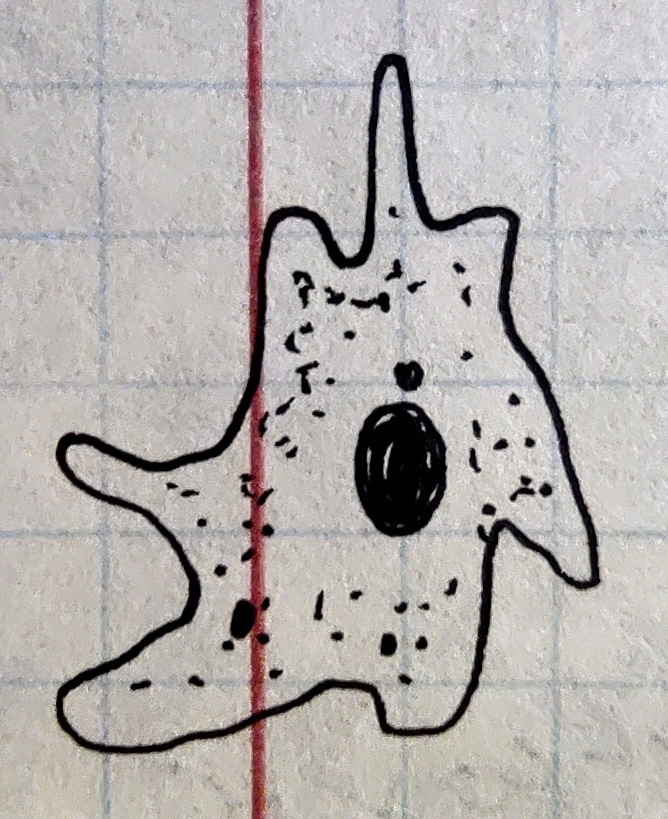
\includegraphics[width=\columnwidth]{ameba_c10_lvl200}
  
      \caption{Не выпуклое.\\{\scriptsize (Рисунок Виолетты Филатовой)}}
    \end{subfigure}
    
    \caption{Линейно связные множества: выпуклое и нет.}
    \label{fig:ameba-and-convex}
  \end{figure}

  \begin{definition}
      Множество $X \hm\subseteq \RR^n$ называется \emph{выпуклым},
      если любую пару точек множества~$X$ можно соединить отрезком (содержащимся во множестве).
  \end{definition}
  
  

  \subsubsection{С3, \S 1, \textnumero 8(1)}

  Для последовательности $\{\bds x^{(m)}\}_{m = 1}^{\infty} \hm\subset \RR^n$ найти предел $\lim_{m \to \infty} \bds x^{(m)}$:
  \[
    \bds x^{(m)} = \left(
      \sqrt{m + 1} - \sqrt{m},\ 
      \frac{m - 1}{m},\ 
      \frac{2m^2 - 1}{m^2},\ 
      \left(1 + \frac{1}{m}\right)^{\! m}
    \right)
  \]
  
  \begin{solution}
    По определению~\eqref{eq:seq-limit}, предел последовательности~$\{\bds x^{(m)}\}_{m = 1}^{\infty} \hm\subset \RR^n$~---~это такой вектор $\bds a \hm\in \RR^n$, что
    \[
      \lim_{m \to \infty} \rho(\bds x^{(m)}, \bds a) = 0
    \]
    или, если подробнее расписать евклидово расстояние между векторами:
    \[
      \lim_{m \to \infty} \sqrt{
        \left(x^{(m)}_1 - a_1\right)^2
        + \left(x^{(m)}_2 - a_2\right)^2
        + \left(x^{(m)}_3 - a_3\right)^2
        + \left(x^{(m)}_4 - a_4\right)^2} = 0
    \]

    Очевидно, что равенство нулю такого предела равносильно одновременному выполнению следующих ``покомпонентных'' равенств с пределами:\footnote{
      В одну сторону равносильность очевидна: если по каждой компоненте последовательность векторов $\{\bds x^{(m)}\}_{m = 1}^{\infty}$ стремится к соответствующей компоненте предельного вектора $\bds a$, то расстояние $\rho(\bds x^{(m)}, \bds a) \hm\to 0$.
      В другую сторону можно доказать от противного: если расстояние между векторами стремится к нулю, но хотя бы по какой-то компоненте ``стремления'' нет, то получается противоречие.
    }\textsuperscript{,}\footnote{
      См. также: С3, \S 1, номер 7.
    }
    \[
      \left\{
        \begin{aligned}
          % &\lim_{m \to \infty} x^{(m)}_1 - a_1 = 0
          &\lim_{m \to \infty} x^{(m)}_1 = a_1\\
          &\lim_{m \to \infty} x^{(m)}_2 = a_2\\
          &\lim_{m \to \infty} x^{(m)}_3 = a_3\\
          &\lim_{m \to \infty} x^{(m)}_4 = a_4
        \end{aligned}
      \right.
    \]

    Таким образом, в качестве предельного вектора имеем:
    \[
      \bds a = \left(
        0, 1, 2, e
      \right)
    \]
  \end{solution}

  
  \subsubsection{Т2}

  Дано множество~(\ref{fig:X-subset-on-R}):
  \[
    X = [1, 2) \cup \{3\} \cup \bigl((4, 5] \cap \QQ\bigr) \subset \RR
  \]

  \begin{figure}[ht]
    \centering
  
    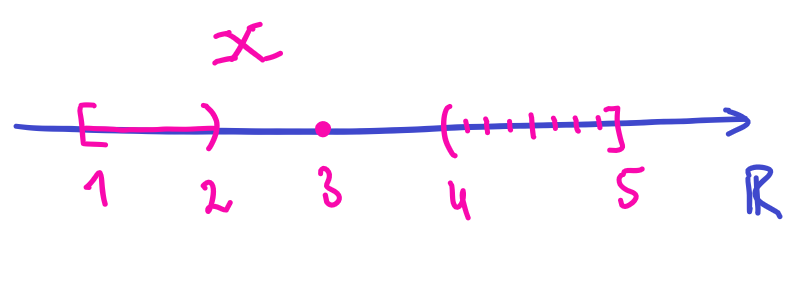
\includegraphics[width=0.5\columnwidth]{X-subset-on-R}
  
    \caption{
      Множество~$X$ на прямой~$\RR$.
    }
    \label{fig:X-subset-on-R}
  \end{figure}

  Надо описать его точки в терминах ``внутренняя'' и т.\,д.
  
  \begin{solution}
    \par\mbox{}
    \begin{enumerate}  % TODO: make as table?
        \item[a)] внутренние точки: $(1, 2)$.
        \item[b)] изолированные точки: $\{3\}$.
        \item[c)] граничные точки: $\{1, 2, 3\} \hm\cup [4, 5]$.
        \item[d)] предельные точки: $[1, 2] \hm\cup [4, 5]$.
        \item[e)] точки прикосновения: $[1, 2] \hm\cup \{3\} \hm\cup [4, 5]$.
    \end{enumerate}

    Граничными точками для~$X$ являются как рациональные, так и иррациональные точки отрезка~$[4, 5]$, потому что в любой окрестности как рационального, так и иррационального числа есть точки обоих типов.
  \end{solution}

  
  \subsubsection{С3, \S 1, \textnumero 14--15}  % two numbers after numero (https://w.wiki/DDF9)

  Пусть $\{G_i\}_{i = 1}^{\infty}$~---~это произвольные открытые в~$\RR^n$ множества.
  Доказать, что в таком случае открытыми будут также следующие множества:
  \[
    \bigcup_{i = 1}^{\infty} G_i,\quad \bigcap_{i = 1}^N G_i
  \]
  (то есть объединение, вплоть до бесконечного числа, открытых множеств открыто; также открыто пересечение, но лишь \emph{конечного} числа открытых множеств).
  
  \begin{solution}
    Как проверить, что объединение открытых открыто?
    Открыто~---~значит, каждая точка должна быть внутренней.
    Пусть некоторый вектор лежит в объединении: $\bds x \hm\in \bigcup_{i = 1}^{\infty} G_i$.
    Тогда он должен быть хотя бы в каком-то из объединяемых множеств: $\exists i^*\colon \bds x \hm\in G_{i^*}$.
    Но раз так, то вектор лежит в этом множестве вместе с какой-то своей окрестностью (раз это множество открыто): $U_{\eps}(\bds x) \hm\subset G_{i^*}$.
    Значит, эта окрестность лежит и в объединении (хоть в конечном, хоть в бесконечном): $U_{\eps}(\bds x) \hm\subset \bigcup_{i = 1}^{\infty} G_i$.

    Аналогичным образом проверим, что пересечение открытых открыто.
    Пусть $\bds x \hm\in \bigcap_{i = 1}^{N} G_i$.
    Это значит, что $\bds x$ принадлежит всем множествам:
    \[
      \left\{
        \begin{aligned}
          &\bds x \in G_i\\
          &i = 1, \ldots, N
        \end{aligned}
      \right.
    \]
    Раз так, то для каждого $G_i$ найдётся окрестность $U_{\eps_i}(\bds x)$ вокруг вектора~$\bds x$, которая целиком лежит в этом $G_i$: $U_{\eps_i}(\bds x) \hm\subset G_i$.
    А так как пересекаемых множеств конечное число, то можно взять \emph{минимальный} из радиусов этих окрестностей:
    \[
      \eps^* = \min\{\eps_1, \ldots, \eps_N\}
    \]
    и окрестность такого радиуса~$U_{\eps^*}(\bds x)$ (или ещё меньшего радиуса) будет находиться во всех пересекаемых множествах: $U_{\eps^*}(\bds x) \hm\subset \bigcap_{i = 1}^{N} G_i$.

    \medskip

    Покажем на примере, что пересечение бесконечного числа открытых множеств не обязательно является открытым.

    Рассмотрим последовательность интервалов на прямой~(\ref{fig:intersection-of-inf-number-opens}):
    \[
      \left\{
        \left(-1 - \frac{1}{n}, 1 + \frac{1}{n}\right)
      \right\}_{n = 1}^{\infty}
    \]

    \begin{figure}[ht]
      \centering
  
      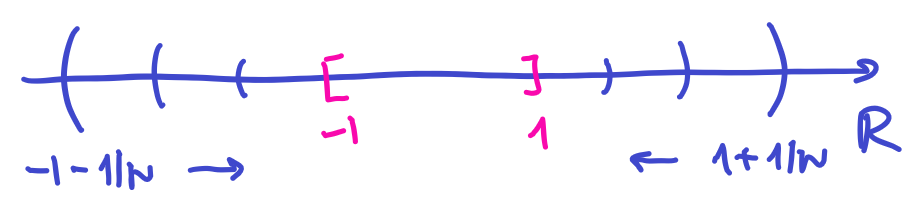
\includegraphics[width=0.5\columnwidth]{intersection-of-inf-number-opens}
  
      \caption{
        Последовательность интервалов $\left\{
          \left(-1 - \frac{1}{n}, 1 + \frac{1}{n}\right)
        \right\}_{n = 1}^{\infty}$ стягивается в отрезок $[-1, 1]$.
      }
      \label{fig:intersection-of-inf-number-opens}
    \end{figure}

    Очевидно, их пересечением будет отрезок:\footnote{
      Указанный отрезок очевидно лежит в пересечении.
      Если допустить, что кроме отрезка в пересечении есть ещё хотя бы одна какая-то точка, то получим противоречие.
      Таким образом, отрезок совпадает с пересечением.
    }
    \[
      \bigcap_{i = 1}^\infty \left(-1 - \frac{1}{n}, 1 + \frac{1}{n}\right) = [-1, 1]
    \]
  \end{solution}


  \subsubsection{С3, \S 2, \textnumero 9(1)}

  Дана функция двух переменных:
  \[
    f(x, y) = \frac{1}{x^2 + y^2 - 1}
  \]
  
  Является ли множество определения функции $f(x, y)$ открытым, замкнутым и т.\,д.?\footnote{
    Более привычный~---~по крайней мере, для кого-то~---~термин ``область определения функции'' намеренно не используется, чтобы избежать ``коллизии'' с другой ``областью''.
  }
  
  \begin{solution}  
    Множество определения функции:
    \[
      x^2 + y^2 - 1 \not= 0 \quad\Leftrightarrow\quad x^2 + y^2 \not= 1
    \]
    представляет собой всю плоскость~$\RR^2$ без окружности радиуса~$1$ около нуля~(\ref{fig:R2-no-circ}).

    \begin{figure}[ht]
      \centering
  
      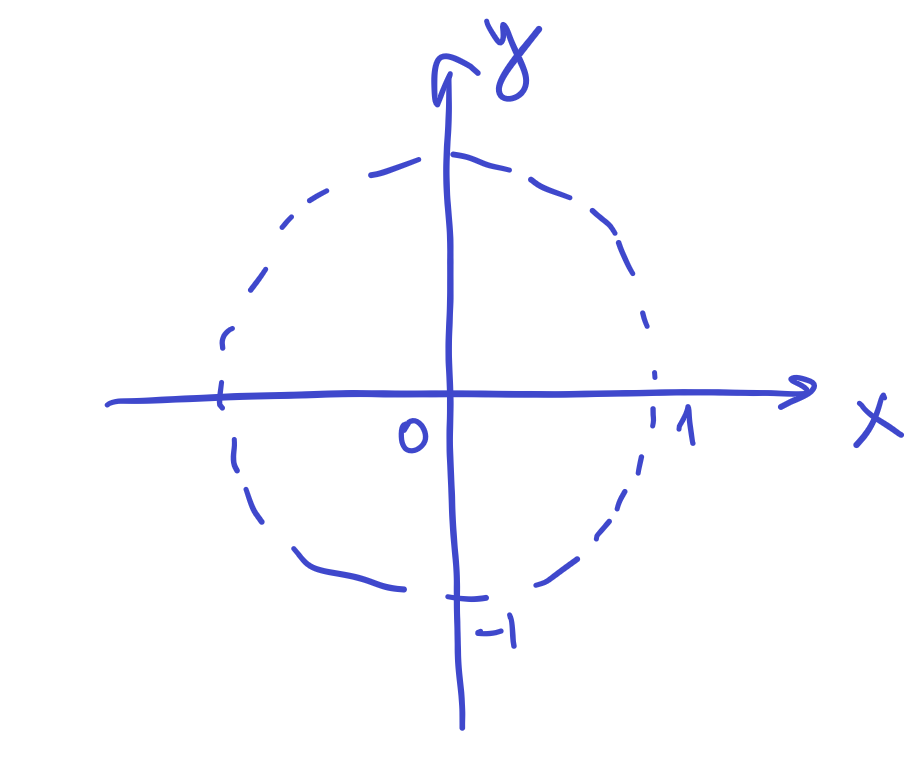
\includegraphics[width=0.5\columnwidth]{R2-no-circ}
  
      \caption{
        $\RR^2 \hm\setminus \{(x, y) \mid x^2 + y^2 = 1\}$.
      }
      \label{fig:R2-no-circ}
    \end{figure}

    Очевидно, такое множество точек на плоскости:
    % \begin{todolist}
    %   \item[\done] открытое
    %   \item[\failed] замкнутое
    %   \item[\failed] линейно связное
    %   \item[\failed] область (= открытое + линейно связное)
    %   \item[\failed] замкнутая область (= область + её замыкание)
    %   \item[\failed] выпуклое
    % \end{todolist}
    \begin{itemize}
      \item открытое
      \item не замкнутое, так как содержит не все точки прикосновения (окружность)
      \item не линейно связное, так как точки внутри и вне круга непрерывной кривой не соединить
      \item не область (= открытое + линейно связное)
      \item не замкнутая область (= область + её замыкание)
      \item не выпуклое (раз какие-то точки не соединить непрерывной кривой, то их не соединить и отрезком)
    \end{itemize}
  \end{solution}


  \subsubsection{Т3}

  Дано множество в пространстве~$\RR^4$:
  \[
    A = \bigl\{
      (x_1, x_2, x_3, x_4) \in \RR^4 \mid x_1^2 + x_2^2 + x_3^2 < x_4^2
    \bigr\}
  \]

  Является ли оно:
  \begin{enumerate}
    \item[a)] открытым
    \item[b)] замкнутым
    \item[c)] областью
  \end{enumerate}
  
  \begin{solution}
    Что из себя представляет множество~$A$?

    При фиксированной координате~$x_4 \hm= r$ получим шар (в оставшихся трёх координатах):
    \[
      x_1^2 + x_2^2 + x_3^2 < r^2
    \]

    Варьируя $x_4 \in \RR$, получаем совокупность шаров.
    Можно думать об этом так: мы живём в трёхмерном пространстве, и четвёртой оси не видим.
    Однако можем каким-то образом перемещаться по этой невидимой оси, и каждый раз при этом видим перед собой новый шар.

    Возможно, стало чем-то понятнее, но вопросы всё равно остаются.
    (Кроме, возможно, вопроса по поводу открытости.)

    Поэтому поступим так.
    Раз в четырёхмерном пространстве множество~$A$ вообразить сложно, посмотрим на ``аналоги''~$A$ в пространствах меньшей размерности.
    Получается, можем начать с плоскости~$\RR^2$.
    ``Двумерная версия''~$A$ определяется так:
    \[
      A = \bigl\{
        (x, y) \in \RR^2 \mid x^2 < y^2
      \bigr\}
    \]

    Условие $x^2 \hm< y^2$ можно, извлёкши\footnote{
      \href{https://w.wiki/DGjC}{Это слово существует}.
    } корень, переписать как $|x| \hm< |y|$.
    Но как изобразить такое~$A$ на плоскости?
    Границы~$A$ задаются условием $|x| \hm= |y|$~---~это две прямые $y \hm= x$ и $y \hm= -x$, которые делят всю плоскость на четверти.
    Отклоняясь с этих прямых равных модулей в какую-либо сторону, можно понять, как изменяется при этом соотношение между модулями $|y|$ и $|x|$.
    В итоге получается, что $A$ состоит из двух четвертей, образующих ``конус'' (без границы)~(\ref{fig:cone-on-plane}).
    Этот конус открыт, но не замкнут, а также не линейно связан (из одной половинки конуса никак не ``пройти'' в другую).

    \begin{figure}[ht]
      \centering
  
      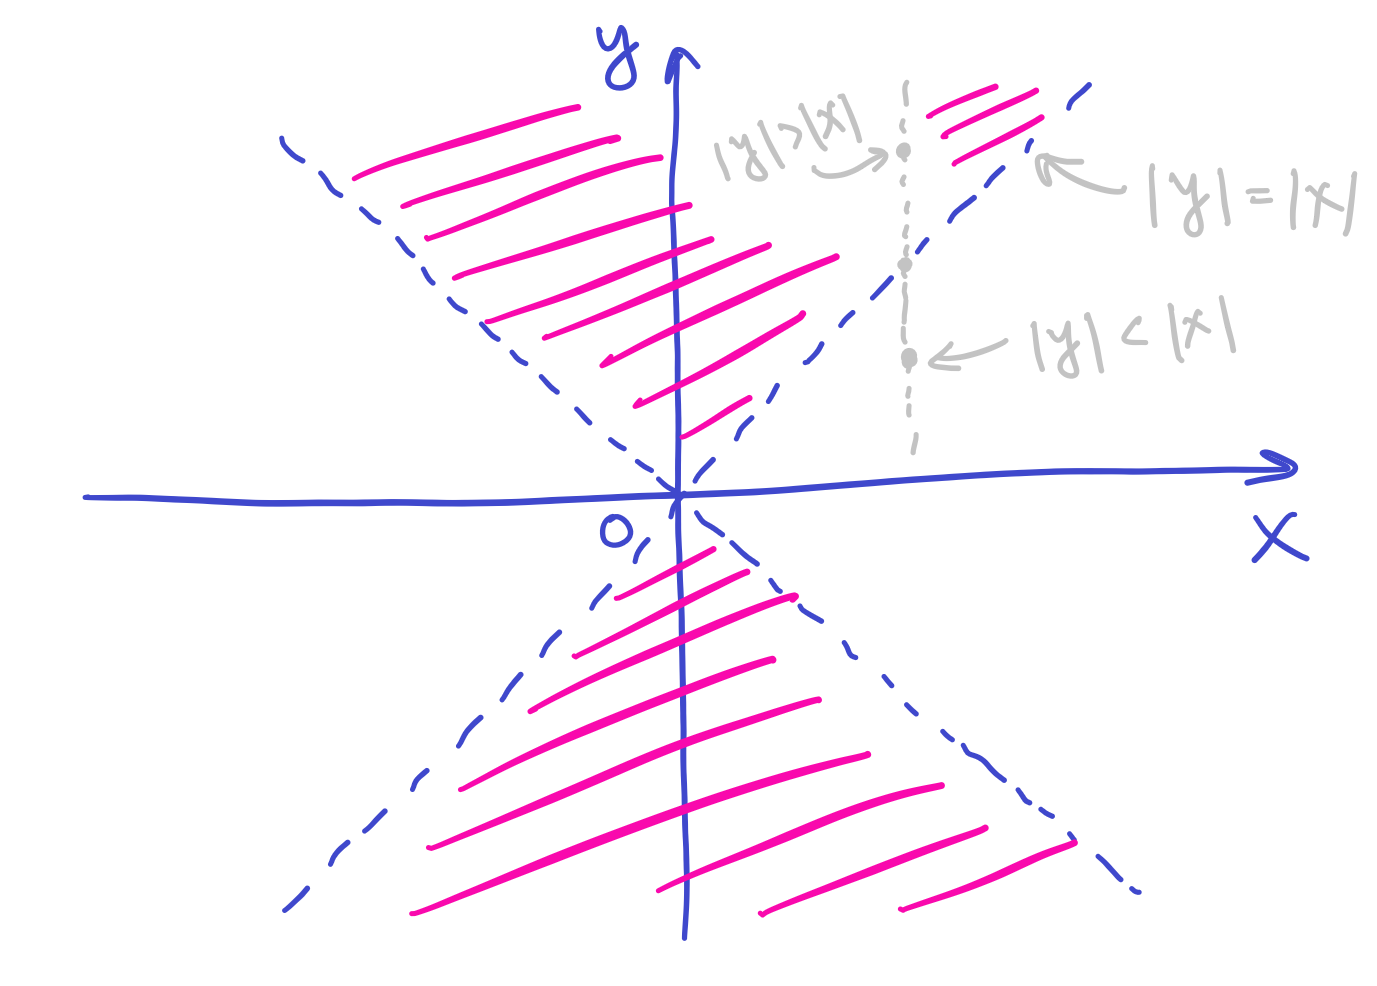
\includegraphics[width=0.8\columnwidth]{cone-on-plane}
  
      \caption{
        ``Конус'' $|y| \hm> |x|$ на плоскости.
      }
      \label{fig:cone-on-plane}
    \end{figure}

    По идее, стоит ожидать, что и четырёхмерный ``аналог''~$A$ будет (не)обладать такими же свойствами (так, из одного шара тоже не попасть в другой, потому что единственная точка, которая могла бы быть связующей, выколота как граничная).
    Но посмотрим ещё на всякий случай на~$A$ в ``трёхмерии'':
    \[
      A = \bigl\{
        (x, y, z) \in \RR^3 \mid x^2 + y^2 < z^2
      \bigr\}
    \]

    Фиксируя и варьируя третью координату, получаем~$A$ как совокупность кругов:
    \[
      A = \bigcup_{r \in \RR} \left\{
        (x, y, z) \in \RR^3 \BigMiddleTwo %\left\{
          \begin{aligned}
            &x^2 + y^2 < r^2\\
            &z = r
          \end{aligned}
        %\right.
      \right\}
    \]
    образующих, как и до этого на плоскости, конус.
    Который, очевидно, также является открытым, но не замкнутым и не линейно связным.

    % TODO: picture of A in 3D
  \end{solution}


  \subsection{О функциях}
  
  О \emph{функции} (отображении) $\phi\colon X \hm\to Y$ можно думать как о правиле,\footnote{
    Источник раздела: \href{https://github.com/Alvant/GeomeSeminare/tree/master2022/seminars/linalge/seminar05}{ЛА 5}.
  } которое \emph{каждому} элементу множества $X$ ставит в соответствие \emph{единственный} элемент множества $Y$\footnote{Множество $X$ в таком случае называется \emph{областью определения} отображения $\phi$ (множество ``допустимых'' входов). Таким образом, область определения~---~это часть определения отображения (определение области определения отображения~---~``тот самый $X$'' из определения отображения). Поэтому, когда в ``школьных'' номерах по математике просили ``найти область определения функции'', то имели в виду найти ``максимально возможное по количеству элементов множество, которое могло бы выступать в роли области определения функции'' (если бы привели полноценное определение этой функции, а не просто формулу).}~(\ref{fig:function}).
  Если отображение $\phi$ переводит элемент $x \hm\in X$ в элемент $y \hm\in Y$, то можно записать $\phi(x) \hm= y$, при этом $y$ называется \emph{образом} $x$, а $x$~---~прообразом $y$ (одним из возможных, если их несколько).
  
  \begin{figure}[ht]
    \centering
  
    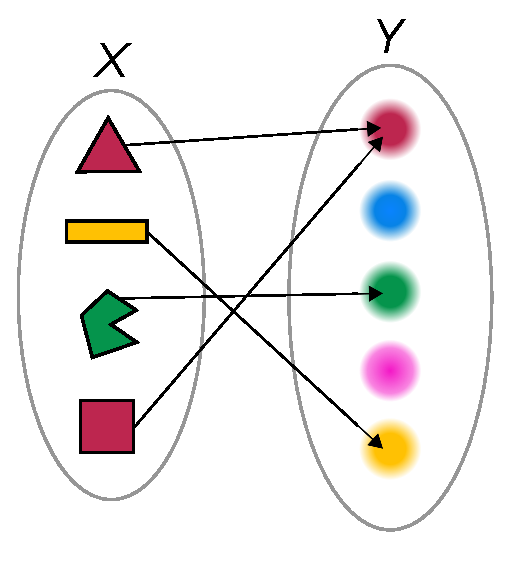
\includegraphics[width=0.3\columnwidth]{function}
  
    \caption{
      Отображение: каждому элементу $X$ соответствует единственный элемент $Y$.
      ({\small \href{https://en.wikipedia.org/wiki/Function\_(mathematics)\#/media/File:Function_color_example_3.svg}{Источник}.})
    }
    \label{fig:function}
  \end{figure}
  
  % Про область определения:
  % https://math.stackexchange.com/a/2912118/451127
  % https://math.stackexchange.com/questions/63043/finding-a-functions-domain-from-the-functions-formula/63048#63048
  
  Можно отметить несколько свойств, которыми могут обладать произвольные отображения.
  
  \begin{definition}
    Отображение~$\phi$ называется \emph{инъективным}, если разные элементы отображаются в разные~(\ref{fig:injection}):
    $
      x_1, x_2 \hm\in X,\ x_1 \hm{\not=} x_2 \hm\Rightarrow \phi(x_1) \hm{\not=} \phi(x_2)
    $.
    Иными словами, если у элемента $y \hm\in Y$ есть прообраз, то он единственный.
  \end{definition}
  
  \begin{definition}
    Отображение~$\phi$ называется \emph{сюръективным}, если у \emph{любого} элемента $y \hm\in Y$ есть прообраз~(\ref{fig:surjection}):
    $
      \forall y \in Y\ \exists x \in X\colon \phi(x) = y
    $.
  \end{definition}
  
  \begin{figure}[ht]
    \centering
    
    \begin{subfigure}[b]{0.3\textwidth}
      \centering
    
      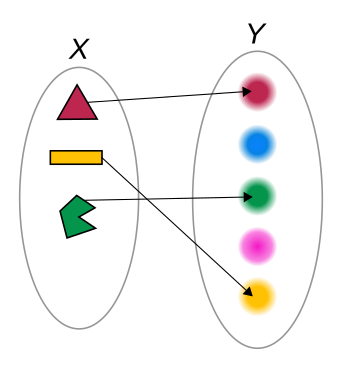
\includegraphics[width=\columnwidth]{injection}
    
      \caption{Инъекция.}
      \label{fig:injection}
    \end{subfigure}
    \hspace{2em}
    \begin{subfigure}[b]{0.3\textwidth}
      
      \centering
      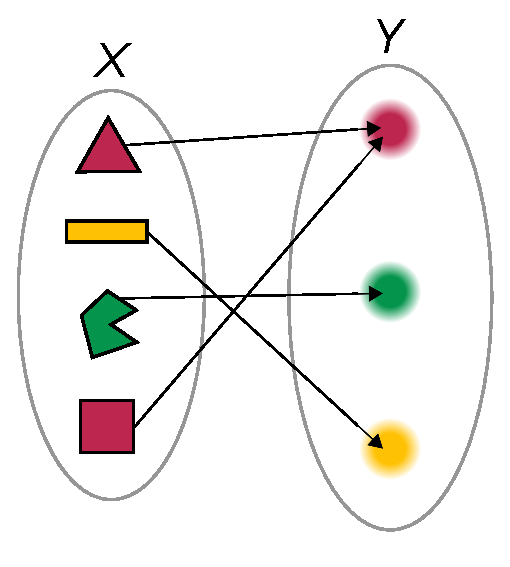
\includegraphics[width=\columnwidth]{surjection}
  
      \caption{Сюръекция.}
      \label{fig:surjection}
    \end{subfigure}
    
    \caption{Инъекция: ``разные в разные'', или ``если есть прообраз, то один''. Сюръекция: ``у~каждого есть хотя бы один прообраз''.}
  \end{figure}
  
  Факт наличия у отображения обоих приведённых выше свойств сразу выделяется в отдельное свойство.
  
  \begin{definition}
    Отображение~$\phi$ называется \emph{биективным}, если у \emph{любого} элемента $y \hm\in Y$ есть \emph{единственный} прообраз:
    $
      \forall y \in Y\ \exists ! x \in X\colon \phi(x) = y
    $.
  \end{definition}
  
  Помимо множества $X$ (области определения отображения $\phi$, или domain), и множества $Y$ (для которого, похоже, в русском языке нет специального названия, а по-английски~---~codomain) можно выделить ещё одно ``интересное'' множество, связанное с отображением~$\phi$~--- это \emph{множество значений} отображения $\Imag \phi \hm\subseteq Y$, которое определяется как совокупность всех элементов $y \hm\in Y$, в которые в принципе ``можно попасть'' под действием отображения:
  \[
    \Imag \phi = \{y \in Y \mid \exists x \in X\colon \phi(x) = y\}
  \]
  
  Тогда сюръективность означает, что $\Imag \phi \hm= Y$.

  
  \subsection{Предел функции}

  % [X] По Коши
  % [X] ПО Гейне

  Введём (обобщим) понятие предела функции для случая функции многих переменных $f\colon X \hm\to \RR$, $X \hm\subseteq \RR^n$.

  Пусть функция $f$ определена в некоторой окрестности точки $\bds x_0$, кроме, возможно, самой $\bds x_0$.\footnote{
    Индекса ``0'' ни у одной координаты вектора нет, поэтому здесь путаницы возникнуть не должно, и будем писать индекс привычным образом снизу.
  }
  (При разговоре о пределе функции в точке важно поведение функции вблизи точки.)

  Число $a$ называется пределом функции $f$ в точке $\bds x_0$ по Коши, если
  \begin{equation}\label{eq:func-limit-cochi}
  \begin{split}
    \forall \eps > 0\ \exists \delta > 0\colon \forall \bds x\colon \left\{
      \begin{aligned}
        &\rho(\bds x, \bds x_0) < \delta\\
        &\bds x \not= \bds x_0
      \end{aligned}
    \right. \to |f(\bds x) - a| < \eps
  \end{split}
  \end{equation}

  Или, то же самое, но немного другими словами:
  \begin{equation}
  \begin{split}
    \forall \eps > 0\ \exists \delta > 0\colon \forall \bds x \in \mathring U_{\delta}(\bds x_0) \to f(\bds x) \in U_{\eps}(a)
  \end{split}
  \end{equation}

  И второй (равносильный) взгляд на предел.

  Число $a$ называется пределом функции $f$ в точке $\bds x_0$ по Гейне, если
  \begin{equation}
  \begin{split}
    \forall \{\bds x^{(m)}\}_{m = 1}^{\infty}\colon \left\{
      \begin{aligned}
        &\lim_{m \to \infty} \bds x^{(m)} = \bds x_0\\
        &\bds x^{(m)} \not= \bds x_0
      \end{aligned}
    \right. \to \lim_{m \to \infty} f\left(\bds x^{(m)}\right) = a
  \end{split}
  \end{equation}
  

  \subsubsection{С3, \S 2, \textnumero 37(8)}

  Дана функция:
  \[
    f(x, y) = x \sin \frac{1}{y} + y \sin \frac{1}{x}
  \]
  
  Найти для неё повторные и ``просто'' пределы:
  \[
    \lim_{x \to 0} \lim_{y \to 0} f(x, y),\quad \lim_{y \to 0} \lim_{x \to 0} f(x, y),\quad \lim_{(x, y) \to (0, 0)} f(x, y)
  \]
  
  \begin{solution}
    При вычислении, например, повторного предела
    \[
      \lim_{x \to 0} \lim_{y \to 0} \left(x \sin \frac{1}{y} + y \sin \frac{1}{x}\right) = \spadesuit
    \]
    надо сначала взять внутренний предел, по одной переменной $y$, считая вторую переменную~$x$ как бы постоянной (и при этом можно считать её отличной от нуля, так как следующим надо будет брать предел при $x \hm\to 0$):  % TODO: sure?
    \[
      \spadesuit = \lim_{x \to 0} \lim_{y \to 0} \left(\pumpkin + 0\right)
      % styx: \olcross
      % ifsym: \BigCross, \Cross
      % https://tug.ctan.org/info/symbols/comprehensive/symbols-a4.pdf
    \]

    Внутренний предел взять не получается.
    С другим повторным пределом будет то же самое.

    Найдём ``просто'' предел.

    \medskip

    \emph{Способ 1: ``Очевидно''}.
    Можно, не долго думая, сразу прийти к выводу, что предел функции в точке $(0, 0)$ будет равен нулю:
    \[
      \lim_{(x, y) \to (0, 0)} \left(x \sin \frac{1}{y} + y \sin \frac{1}{x}\right) = 0
    \]
    просто потому что оба слагаемых при одновременном стремлении $x \to 0$ и $y \to 0$ также стремятся к нулю.

    \medskip

    \emph{Способ 2: ``Модуль за скобку''} (отсылка к $\CC$).
    Немного преобразуем выражение под пределом, вынеся за скобку корень $\sqrt{x^2 + y^2}$:
    \[
      \lim_{(x, y) \to (0, 0)} \left(x \sin \frac{1}{y} + y \sin \frac{1}{x}\right) = \lim_{(x, y) \to (0, 0)} \sqrt{x^2 + y^2}\left(\frac{x}{\sqrt{x^2 + y^2}} \cdot \sin \frac{1}{y} + \frac{y}{\sqrt{x^2 + y^2}} \cdot \sin \frac{1}{x}\right)
    \]

    Что таким образом получаем: множитель $\sqrt{x^2 + y^2} \hm\to 0$.\footnote{
      Потому что одновременное стремление $x \hm\to 0$ и $y \hm\to 0$ по сути и равносильно стремлению $\sqrt{x^2 + y^2} \hm\to 0$.
      Или же можно сказать, что это просто следует из определения: $(x, y) \hm\to (0, 0) \hm\Leftrightarrow \rho\bigl((x, y), (0, 0)\bigr) \hm\to 0$
    }
    Оставшаяся же ``скобка'' ограничена: $\frac{x}{\sqrt{x^2 + y^2}}$ и $\frac{y}{\sqrt{x^2 + y^2}}$ могут быть синусом и косинусом некоторого угла, в результате в скобках получается что-то в духе развёрнутого синуса или косинуса суммы.
    И всё выражение стремится к нулю.

    \medskip

    \emph{Способ 3: По определению}.

    Из здравого смысла понимаем, что предел функции в нуле~---~это, скорее всего, ноль.
    Докажем теперь это по определению~\eqref{eq:func-limit-cochi}.

    Функция сходится к нулю в точке $(0, 0)$, если:
    \[
      \forall \eps > 0\ \exists \delta\colon \forall \bds x \colon 0 < \rho(\bds x, \bds 0) < \delta \to |f(\bds x) - 0| < \eps
    \]
    где $\bds x \hm= (x, y)$ и $\rho(\bds x, \bds 0) \hm= \sqrt{x^2 + y^2}$.

    Начнём расписывать (оценивать сверху) $|f(\bds x)|$ (в расчёте прийти в итоге к выражению, где можно будет воспользоваться какой-угодно-малостью $\sqrt{x^2 + y^2}$):
    \[
      |f(\bds x)| = \left|x \sin \frac{1}{y} + y \sin \frac{1}{x}\right| = \spadesuit
    \]

    Вынесем расстояние $\rho(\bds x, \bds 0)$ ``за скобку'':
    \[
      \spadesuit = \sqrt{x^2 + y^2} \cdot \left|\frac{x}{\sqrt{x^2 + y^2}} \cdot \sin \frac{1}{y} + \frac{y}{\sqrt{x^2 + y^2}} \cdot \sin \frac{1}{x}\right| \leq \diamondsuit
    \]

    Что можно сказать про сумму под модулем?
    % Синус и косинус ни к чему не сходятся (скачут от $-1$ до $1$), но они ограничены.
    % Множители же $\frac{x}{\sqrt{x^2 + y^2}}$ и $\frac{y}{\sqrt{x^2 + y^2}}$~---~это тоже в некотором смысле косинус и синус какого-то угла (см. похожий сюжет в теме про комплексные числа ранее в конспектах).
    % Таким образом, сумма в скобках ограничена (на неё даже можно смотреть как на косинус или синус суммы углов).
    То же, что и раньше~---~на неё можно смотреть как на синус суммы углов, и она ограничена.
    И эта скобка умножается на $\sqrt{x^2 + y^2}$, который может быть сделан сколь угодно малым.
    Хочется же в итоге получить $|f(\bds x)| \hm< \eps$: 
    \[
      \diamondsuit \leq \delta \cdot 1 < \eps
    \]

    Выходит, $\forall \eps \hm> 0$ найдётся $\delta \hm< \eps$ (например, $\delta \hm= \eps \hm/ 2$), при котором $|f(\bds x)| \hm< \eps$ для всех $\bds x$, таких что $\sqrt{x^2 + y^2} \hm< \delta$.
    Таким образом, в самом деле $\lim_{(x, y) \to (0, 0)} f(x, y) \hm= 0$.

    \medskip

    \emph{Способ 4: Графический}.
    
    В дополнение к аналитическим (``формульным'') решениям можно ещё посмотреть на картинку (\ref{fig:plot_3d}).

    \begin{figure}[ht]
      \centering
  
      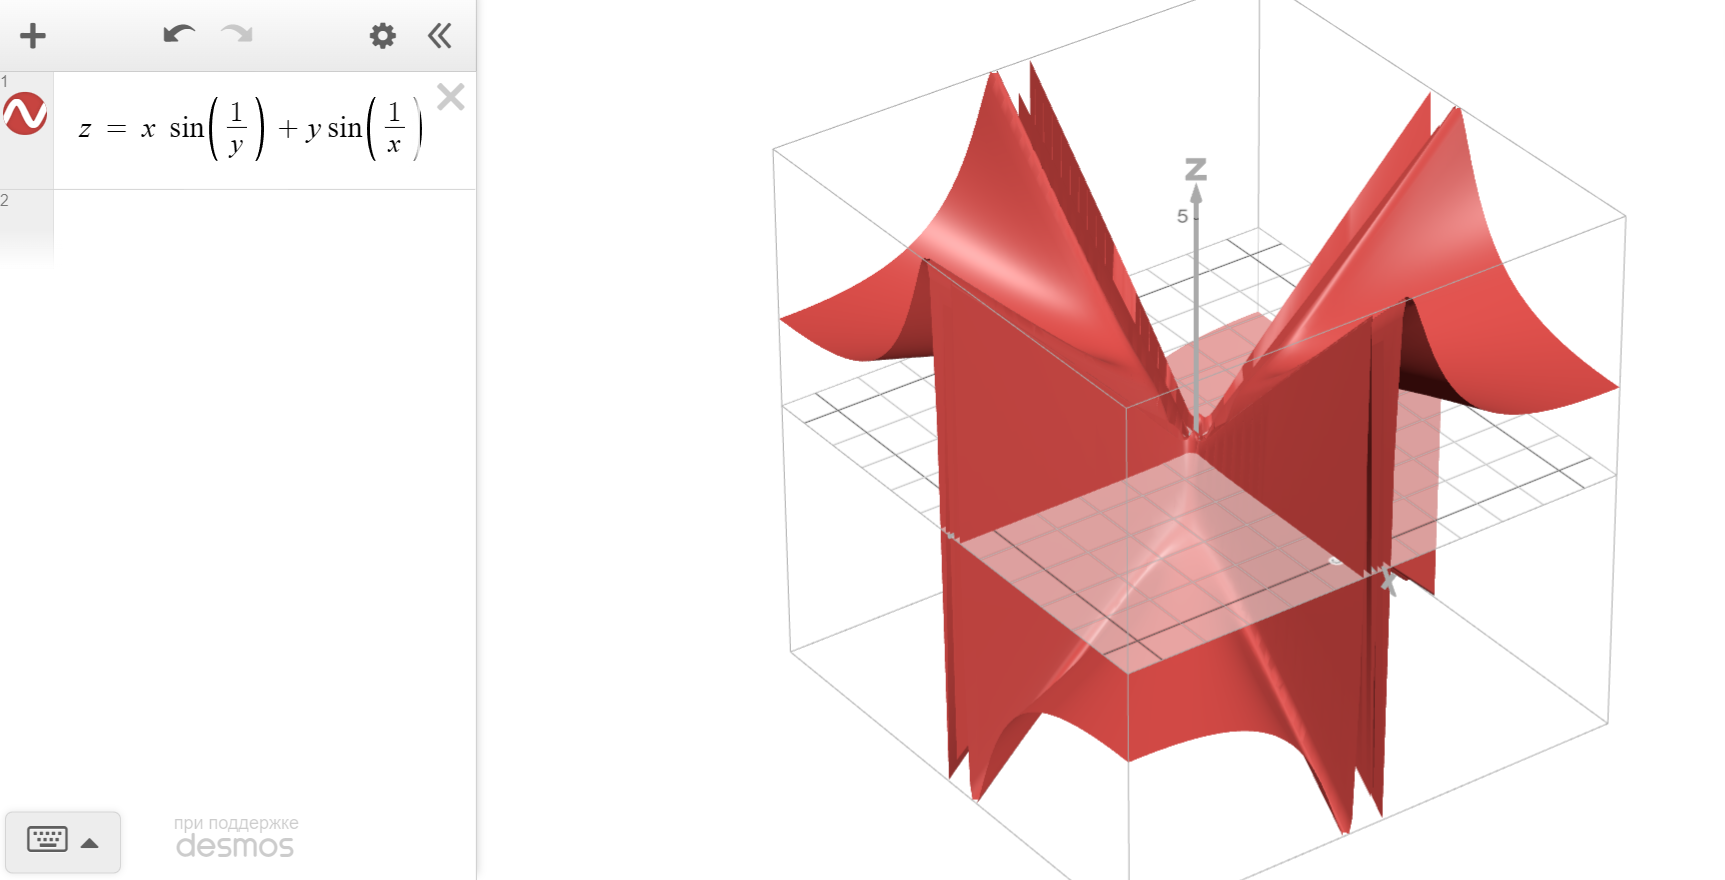
\includegraphics[width=0.8\columnwidth]{plot_3d}
  
      \caption{
        \href{https://www.desmos.com/3d}{График} функции $z \hm= x \sin \frac{1}{y} + y \sin \frac{1}{x}$.
      }
      \label{fig:plot_3d}
    \end{figure}
    
    Видно, что если, например, зафиксировать (вообще никак не трогать) переменную $y$, а двигаться к нулю только по $x$, то ни к чему сойтись не получится.
    Поэтому повторных пределов в нуле нет.
    Двигаться к нулю надо одновременно по обеим переменным.
  \end{solution}


  \subsubsection{С3, \S 2, \textnumero 48(7)}

  Найти предел функции $f(x, y)$ в точке:
  \[
    \lim_{(x, y) \to (0, 0)} \sqrt{x^2 + y^2} \ln (x^2 + y^2)
  \]
  
  \begin{solution}
    % TODO: Если есть предел -- повторные с ним совпадают?
    % Ответ: нет -- смотри решение одного из номеров в этом же конспекте (про x sin (1/y) + y sin (1/x))

    Для простоты (и чтобы получить некоторую ``интуицию'') рассмотрим предел, например, вдоль прямой $y \hm= x$:
    \[
      \lim_{\substack{x \to 0\\ y = x}} \sqrt{x^2 + y^2} \ln (x^2 + y^2) = \lim_{x \to 0} \sqrt{2 x^2} \ln (2 x^2) = \spadesuit
    \]

    Далее, можно ещё заменить $\sqrt{2x^2} \hm\equiv t \hm\geq 0$ (хотя можно бы было и без этого):
    \[
      \spadesuit = \lim_{t \to +0} t \ln t^2 = 2 \lim_{t \to +0} \frac{\ln t}{1/t} = 0
    \]
    где равенство нулю в конце можно доказать с помощью правила Лопиталя.

    Таким образом, гипотеза, что:
    \[
      \lim_{(x, y) \to (0, 0)} \sqrt{x^2 + y^2} \ln (x^2 + y^2) = 0
    \]

    Как это доказать?
    Можно заметить, что... в этом пределе от двух переменных тоже можно сделать замену!
    Положим $t \hm\equiv x^2 \hm+ y^2 \hm\geq 0$.
    Тогда стремление $(x, y) \hm\to (0, 0)$ будет равносильно $t \hm\to 0+$, и предел перепишется следующим образом:
    \[
      \lim_{t \to 0+} \sqrt{t} \ln t
    \]

    А предел такого вида уже как раз находили выше.
  \end{solution}


  \subsubsection{С3, \S 2, \textnumero 62(5)}

  Найти все точки разрыва (устранимого и нет) функции двух переменных:
  \[
    f(x, y) = \left\{
      \begin{aligned}
        &\frac{x^3 + y^3}{x + y}, & &\mbox{если}\ x + y \not= 0\\
        &\ 3,                       & &\mbox{если}\ x + y = 0
      \end{aligned}
    \right.
  \]
  
  \begin{solution}
    To be continued...
  \end{solution}

  % TODO:
  % \subsection{Частные произфодные. Дифференциал}

  % \subsubsection{С3, \S 3, \textnumero 12}
  
  % \begin{solution}
  % \end{solution}


  % \subsubsection{С3, \S 3, \textnumero 15(7)}
  
  % \begin{solution}
  % \end{solution}


  % \subsubsection{С3, \S 3, \textnumero 19(2)}
  
  % \begin{solution}
  % \end{solution}
\end{document}
